\documentclass[a4paper, tikz, border=10pt]{article}

% necessary package
\usepackage[english]{babel}
\usepackage[utf8]{inputenc}
\usepackage[colorinlistoftodos]{todonotes}
\usepackage{parskip} % spacing between paragraphs controller
\usepackage{amsmath} % equation alignment and reference
\usepackage{enumerate} % list items
\usepackage{graphicx} % figure alignment and reference

%% algorithm pseudocode related
% \usepackage{algorithmicx}
% \usepackage[noend]{algpseudocode}
% \usepackage[linesnumbered, ruled, vlined]{algorithm2e}

%% automata circle and edges related
% \usepackage{tikz}
% \usetikzlibrary{automata,positioning}

% other package
\usepackage{amssymb} % empty set package
\usepackage{url} % url reference
\usepackage{multirow} % multiple rows/columns in table

% insert c code
\usepackage{xcolor}
\usepackage{listings}
\definecolor{mGreen}{rgb}{0,0.6,0}
\definecolor{mGray}{rgb}{0.5,0.5,0.5}
\definecolor{mPurple}{rgb}{0.58,0,0.82}
\definecolor{backgroundColour}{rgb}{0.95,0.95,0.92}

\lstdefinestyle{CStyle}{
    backgroundcolor=\color{backgroundColour},   
    commentstyle=\color{mGreen},
    keywordstyle=\color{magenta},
    numberstyle=\tiny\color{mGray},
    stringstyle=\color{mPurple},
    basicstyle=\footnotesize,
    breakatwhitespace=false,         
    breaklines=true,                 
    captionpos=b,                    
    keepspaces=true,                 
    numbers=left,                    
    numbersep=5pt,                  
    showspaces=false,                
    showstringspaces=false,
    showtabs=false,                  
    tabsize=2,
    language=C
}

\usepackage{tikz}
\usetikzlibrary{positioning}
\tikzset{
  gray box/.style={
    fill=gray!20,
    draw=gray,
    minimum width={2*#1ex},
    minimum height={2em},
  },
  annotation/.style={
    anchor=north,
  }
}

% change to a new line when necessary
\makeatletter 
\def\UrlAlphabet{%
      \do\a\do\b\do\c\do\d\do\e\do\f\do\g\do\h\do\i\do\j%
      \do\k\do\l\do\m\do\n\do\o\do\p\do\q\do\r\do\s\do\t%
      \do\u\do\v\do\w\do\x\do\y\do\z\do\A\do\B\do\C\do\D%
      \do\E\do\F\do\G\do\H\do\I\do\J\do\K\do\L\do\M\do\N%
      \do\O\do\P\do\Q\do\R\do\S\do\T\do\U\do\V\do\W\do\X%
      \do\Y\do\Z}
\def\UrlDigits{\do\1\do\2\do\3\do\4\do\5\do\6\do\7\do\8\do\9\do\0}
\g@addto@macro{\UrlBreaks}{\UrlOrds}
\g@addto@macro{\UrlBreaks}{\UrlAlphabet}
\g@addto@macro{\UrlBreaks}{\UrlDigits}
\makeatother

\setlength{\parindent}{0pt} % no indent in the beginning of a paragraph


\title{CSCE 451/851 Homework 4}
\author{Tian Gao}
\begin{document}
\maketitle

% ! Q1
Q1. \\
a.\\
It is possible that more than 3 processes are active.\\
For example, let's assume there are old processes leaving, 3 processes (A, B, C) are waiting for block in L9, and 1 process (D) is waiting for mutex in L5.
As the old processes leave, A, B, C comes to L10 and must\_wait is still false.
Then D is unblocked and comes to L19.
Then ABC are unblocked and come to L19 one by one.
As a result, there are four processes coming to L19 at the same time, which proves the incorrectness of the program.

b.\\
Yes. Changing if to while will solve the problem.\\
The problem is the potential starvation of the waiting processes since the new processes are easier to come to the critical section comparing to the waiting ones.

c.\\
The problem can be solved by moving L10 before L13.\\
If L10 is moved, new processes will also semWait(block). 
Then only three processes are able to come to L19 at the same time.

% ! Q2
Q2. \\
\begin{lstlisting}[style=CStyle]
    /* Include Files */
    #include <pthread.h>
    #include <stdio.h>
    
    /* External References */
    extern int world(void);
    extern int hello(void);
    extern int exclamation(void);
    void *threadCall1(void *arg);
    void *threadCall2(void *arg);
    void *threadCall3(void *arg);
    
    int main(int argc, char *argv[])
    {
        pthread_t thread[3];
    
        pthread_create(&thread[0], NULL, threadCall1, NULL);
        pthread_join(thread[0], NULL);
    
        pthread_create(&thread[1], NULL, threadCall2, NULL);
        pthread_join(thread[1], NULL);
    
        pthread_create(&thread[2], NULL, threadCall3, NULL);
        pthread_join(thread[2], NULL);
    
        printf("\n");
        pthread_exit(NULL);
        return (0);
    }
    
    void *threadCall1(void *arg)
    {
        hello();
    }
    
    void *threadCall2(void *arg)
    {
        world();
    }
    
    void *threadCall3(void *arg)
    {
        exclamation();
    }
    
    /* world - print the "world" part. */
    int world(void)
    {
        printf("world");
        return 0;
    }
    
    /* hello - print the "hello" part. */
    int hello(void)
    {
        printf("hello ");
        return 0;
    }
    
    /* exclamation - print "!".*/
    int exclamation()
    {
        printf("!");
        return 0;
    }
\end{lstlisting}

Execution result on CSE server:\\

\centerline{\includegraphics[width=0.8\textwidth]{fig/q2.png}}

% ! Q3
Q3.\\
a.\\
FCFS:\\
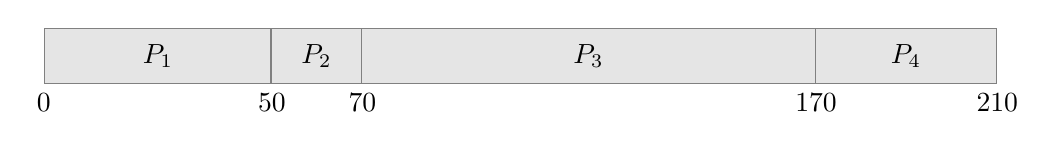
\begin{tikzpicture}[node distance=-0.5pt]
    \node [gray box=50/210*40] (p1) {\(P_{1}\)};
    \node [gray box=20/210*40, right=of p1] (p2) {\(P_{2}\)};
    \node [gray box=100/210*40, right=of p2] (p3) {\(P_{3}\)};
    \node [gray box=40/210*40, right=of p3] (p4) {\(P_{4}\)};

    \node [annotation] at (p1.south west) {0};
    \node [annotation] at (p1.south east) {50};
    \node [annotation] at (p2.south east) {70};
    \node [annotation] at (p3.south east) {170};
    \node [annotation] at (p4.south east) {210};
\end{tikzpicture}

non-preemptive priority:\\
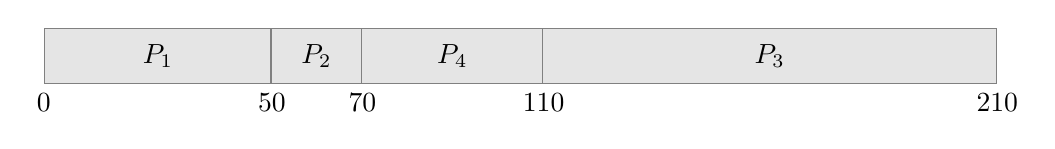
\begin{tikzpicture}[node distance=-0.5pt]
    \node [gray box=50/210*40] (p1) {\(P_{1}\)};
    \node [gray box=20/210*40, right=of p1] (p2) {\(P_{2}\)};
    \node [gray box=40/210*40, right=of p2] (p3) {\(P_{4}\)};
    \node [gray box=100/210*40, right=of p3] (p4) {\(P_{3}\)};

    \node [annotation] at (p1.south west) {0};
    \node [annotation] at (p1.south east) {50};
    \node [annotation] at (p2.south east) {70};
    \node [annotation] at (p3.south east) {110};
    \node [annotation] at (p4.south east) {210};
\end{tikzpicture}

round robin:\\
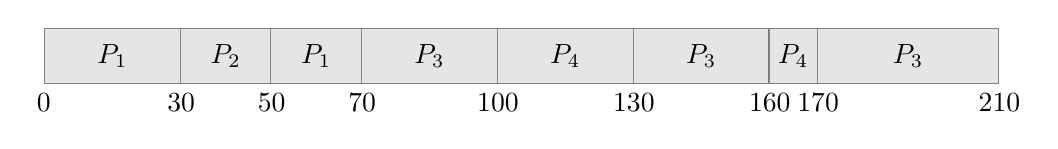
\begin{tikzpicture}[node distance=-0.5pt]
    \node [gray box=30/210*40] (p1) {\(P_{1}\)};
    \node [gray box=20/210*40, right=of p1] (p2) {\(P_{2}\)};
    \node [gray box=20/210*40, right=of p2] (p3) {\(P_{1}\)};
    \node [gray box=30/210*40, right=of p3] (p4) {\(P_{3}\)};
    \node [gray box=30/210*40, right=of p4] (p5) {\(P_{4}\)};
    \node [gray box=30/210*40, right=of p5] (p6) {\(P_{3}\)};
    \node [gray box=10/210*40, right=of p6] (p7) {\(P_{4}\)};
    \node [gray box=40/210*40, right=of p7] (p8) {\(P_{3}\)};

    \node [annotation] at (p1.south west) {0};
    \node [annotation] at (p1.south east) {30};
    \node [annotation] at (p2.south east) {50};
    \node [annotation] at (p3.south east) {70};
    \node [annotation] at (p4.south east) {100};
    \node [annotation] at (p5.south east) {130};
    \node [annotation] at (p6.south east) {160};
    \node [annotation] at (p7.south east) {170};
    \node [annotation] at (p8.south east) {210};
\end{tikzpicture}

b.\\
FCFS:\\
waiting time of $P_{1}$: 0 ms.\\
waiting time of $P_{2}$: 70 - 20 - 20 = 30 ms.\\
waiting time of $P_{3}$: 170 - 100 - 40 = 30 ms.\\
waiting time of $P_{4}$: 210 - 40 - 60 = 110 ms.\\
average waiting time: 42.5 ms.

non-preemptive priority:\\
waiting time of $P_{1}$: 0 ms.\\
waiting time of $P_{2}$: 70 - 20 - 20 = 30 ms.\\
waiting time of $P_{3}$: 210 - 100 - 40 = 70 ms.\\
waiting time of $P_{4}$: 110 - 40 - 60 = 10 ms.\\
average waiting time: 27.5 ms.

round robin:\\
waiting time of $P_{1}$: 70 - 50 = 20 ms.\\
waiting time of $P_{2}$: 50 - 20 - 20 = 10 ms.\\
waiting time of $P_{3}$: 210 - 100 - 40 = 70 ms.\\
waiting time of $P_{4}$: 170 - 40 - 60 = 70 ms.\\
average waiting time: 42.5 ms.

c.\\
FCFS:\\
turnaround time of $P_{1}$: 50 ms.\\
turnaround time of $P_{2}$: 70 - 2 ms.0 = 50\\
turnaround time of $P_{3}$: 170 - 40 = 130 ms.\\
turnaround time of $P_{4}$: 210 - 60 = 150 ms.\\
average turnaround time: 95 ms.

non-preemptive priority:\\
turnaround time of $P_{1}$: 50 ms.\\
turnaround time of $P_{2}$: 50 ms.\\
turnaround time of $P_{3}$: 210 - 40 = 170 ms.\\
turnaround time of $P_{4}$: 110 - 60 = 50 ms.\\
average turnaround time: 80 ms.

round robin:\\
turnaround time of $P_{1}$: 70 ms.\\
turnaround time of $P_{2}$: 50 - 20 = 30 ms.\\
turnaround time of $P_{3}$: 210 - 40 = 170 ms.\\
turnaround time of $P_{4}$: 170 - 60 = 110 ms.\\
average turnaround time: 95 ms.

% ! Q4
Q4.\\
a. I/O first half, processor second half. \\
one job:\\
Turnaround time: NT\\
Throughput: $\frac{1}{N}$\\
Processor utilization: 50\%\\

two jobs:\\
Turnaround time: NT\\
Throughput: $\frac{2}{N}$\\
Processor utilization: 100\%\\

four jobs:\\
Turnaround time: (2N - 1)T\\
Throughput: $\frac{4}{N}$\\
Processor utilization: 100\%\\

b. I/O first and fourth quarters, processor second and third quarter. \\
one job:\\
Turnaround time: NT\\
Throughput: $\frac{1}{N}$\\
Processor utilization: 50\%\\

two jobs:\\
Turnaround time: NT\\
Throughput: $\frac{2}{N}$\\
Processor utilization: 100\%\\

four jobs:\\
Turnaround time: (2N - 1)T\\
Throughput: $\frac{4}{N}$\\
Processor utilization: 100\%\\

% ! Q5
Q5.\\
a.\\
The times for which the process is selected and executed will be doubled.

b.\\
The processes of importance will have more execution time and can be completed sooner.

c.\\
We can achieve the same effect using the quantum with a variable length in RR algorithm.
The length of quantum depends on the priority of the process.

\end{document}
